\chapter{Internet Of Things}
\label{chapter:internetofthings} 

\section{Things: Bridging The Real and The Virtual World}

The term, Internet of Things, was firstly mentioned by Kevin Ashton in once his presentation in 1999 \cite{ashton2009internet}.

Semantically, Internet of Things means ``a world-wide network of interconnected objects uniquely addressable, based on standard communication protocols'' \cite{infso2008networked}. 

The ``things'' refers to the ``objects'' in the semantical explanation. The ``things'' are heterogeneous objects. The initial idea of the ``things'' started with Radio-Frequency IDentification (RFID) tags by Auto-ID Labs\footnote{http://www.autoidlabs.org}, a world-wide network of academic research laboratory in the field of networked RFID and emerging sensing technologies. Hereafter, other concepts of ``things'' emerged: NFC tags, Wireless Sensor and Actuator Networks (WSANs), Spime and Smart Items.

\subsection{NFC and WSANs}

NFC is a proximity technology that provides contactless communication by using ISO/IEC 14443 and ISO/IEC 18092. NFC tags utilise Reader/Writer mode, one of the modes that a NFC devices should supports \cite{Madlmayr:SecurityandPrivacy}, to store data and interact with users. A typical scenario is that a NFC tag acts as a smart poster, where a user could place a NFC based mobile phone near a smart poster and thus would retrieve further information. For instance, if a smart poster stores movie poster data, it can forward a user to the movie trailer or its home page. Additionally, there are card emulation mode and Peer-to-Peer mode. Card Emulation Mode e.g. turns a mobile phone into a smart card such as a credit or debit card, and the NFC reader cannot distinguish the difference between the mobile phone and smart cards. Thus, with this features, it can implement a new way of payment system called Mobile Payments. NFC Peer-to-Peer (P2P) mode is designed based on the standards ISO 18092, which allows two NFC devices communicate mutually \cite{Madlmayr:SecurityandPrivacy}.

WSANs are composed of large numbers of minimal capacity sensing, computing, and communicating devices and various types of actuators. WSANs constitute an important and exciting new technology with great potential for improving many current applications. It also creates new revolutionary systems in areas such as global-scale environmental monitoring, precision agriculture, home and assisted living medical care, smart buildings and cities, industrial automation, and numerous military applications \cite{stankovic2008sensor}. 

They are, together with RFID, are recognised as the atomic components that links the real world with the digital world \cite{sterling2005shaping}.

\subsection{Spime and Smart Items}

Spime and Smart Items are also considered to be the ``things''. Spime is a neologism created by Bruce Sterling, a science fiction writer, in 2005. Sterling stated that there will be a new kind of object -- user-alterable, baroquely multi-featured and programmable -- in the future, for which Sterling invented the term ``Spime'' \cite{sterling2005shaping}. Sterling described that the Spime is one of the objects in Internet of Things since Spime enables a thing to be searchable. i.e. A thing can be searched by a search engine from a virtual world to a physical world \cite{sterling2005shaping}. Spime is a bit theoretical, but we can find some of its prototype in the real world, and we call them Smart Items \cite{atzori2010internet}.

IoT is also derivative from the vision of ``Internet'', which Vasseur and Adam described in \cite{vasseur2010interconnecting}. A Smart Object is an item equipped with a form of sensor or actuator, a tiny microprocessor, a communication device and a power source. The sensor or actuator gives the smart object the ability to interact with the physical world. Smart Objects are interconnected using the Internet Protocol (IP). 

According to IPSO Alliance, the IP stack is a light protocol that already connects a huge amount of communicating devices and runs on tiny and battery operated embedded devices. This guarantees that IP has all the qualities to make IoT a reality \cite{atzori2010internet}.

\section{Sensors and Actuators}
A sensor detects or measures the physical environment (such as temperature, speed, and location etc) and converts it to a form (such as a digital form) which can be read by human or used for other purpose. For example, a light sensor senses the brightness of the environment, then the sensor converts the brightness into a digital form (data). The data can be, further, transferred to other receivers.

Sensors can interconnect wirelessly, and form a network, which is called wireless sensor network (WSN). WSN monitors the environment or other physical data distributively. According to \cite{culler2004guest}, WSN can be apply to a wide range of uses: monitoring space, things, and the encompassing space. Particularly, the first category, space, which is related to the thesis, covers light, temperature, humidity and other environment data. 

Sensors perform tasks more than measuring environments. The second category applies on things or objects. Sensors, that being the case, are applied more in area of such as, the detection of structures breakages \cite{christin2009wireless}. However, things and the environment are sometimes interconnected and interactive. This is the third category when sensors are used to e.g. monitor the wildlife habitats \cite{culler2004guest} and the interaction between traffic queuing and the frequency of traffic lights switching. In short, the WSN provides a good source of data for Internet of Things.

Sensors collect and transfer data for further use, but an actuator provides controlling functions to a system. e.g. a light switch can turn on and turn off a light; Here the light switch is an actuator. Sensors and Actuators work mutually can optimise processes. For example, sensors are installed in chemical production to bring much greater granularity to monitoring, where the sensor collects data and transfers them to computers which subsequently analyse the data and signal actuators to adjust the processes, such as ingredient mixtures, temperatures, or pressures \cite{chui2010internet}. The whole process can then be automated. 

\section{Internet-based Communication Protocols and Standards with IoT}
The currently architecture of IoT consists three layers \cite{wu2010research}. From top to bottom, they are: application layer, network layer and perception layer. The perception layer consists of the unquietly addressable objects. The network layer connects the objects and connects objects to computers. The application layer makes the IoT data meaningful, useful or extensible.

TCP/IP and UDP ensure the objects communicable in IoT. Moreover, they ensure that the objects can be communicated outside the IoT network. Subsequently, the data, e.g. that sensors collected, is utilisable. For example, the data collected by sensors can be transferred to a data centre and can be further analysed. 

Another issue about IP, Internet Protocol Version 4 (IPv4) is the dominant IP protocol in the Internet currently. IPv4, however, has exhausted \cite{smith2011free} and thus could not meet the `unquietly addressable' requirement in IoT. IP Version 6 (IPv6) is its successor. ``IPv6 enables end-to-end communication, in which any IPv6 `smart things' can connect to any other IPv6 devices or system from any place and at any time. It enables the possible extension of the Internet to any device, sensor or actuator, which can become real nodes of the future Internet.'' \cite{vermesan2011internet}. It primarily provides the following features\cite{deering1998internet}: 

\begin{itemize}
% You can use this command to set the items in the list closer to each other
% (ITEM SEParation, the vertical space between the list items) 
\setlength{\itemsep}{0pt}
\item Expanding addressing capabilities to support a greater amount of addressable nodes. 
\item Simplifying header format to reduce the cost of packet handling.
\item Improving support for extensions and options to allow greater flexibility in the future
\item Flowing labelling capability to label packets and thus to handle, e.g., real-time services.
\item Authentication and privacy capabilities
\end{itemize}

HTTP and WebSocket ensure that IoT can be used or extended by applications. For example, a web interface that can visualise temperature data. Subsequently, IoT network can be directly or indirectly connect to end users. 

A Web Service ``is a network accessible interface to application functionality, built using standard Internet technologies'' \cite{snell2009programming}. In other words, an application can be accessed by another application, client or user over the Internet, via web technology such as HTTP, XML or SMTP. A Web Service, usually, provides services based on standards at the layer between service requesters and service providers. This means, it does not matter how are the services implemented, e.g. using C/C++, Java, Python or Javascript, or based on whatever platforms, e.g. Windows Server, Max OS Server or Unix Server. 

When a request is sent to a web service layer, this layer will start a procedure which further requests the service provider. When the procedure is finished, the web service layer will response to the sender results (the response is sometimes optional and it relies on how is the web service implemented). The communication, between the service requesters and the web service layer, is usually based on standard protocols, which aims at cross-platform interoperability. 

The next, we will talk about a sequence of protocols that can be used in Web Services.

\subsection{REST}
Representational State Transfer (REST) is introduced by ROY T. FIELDING in his doctoral dissertation in 2000. REST is a web architectural style. It is, however, not a standard or protocol. 

An architectural style is ``a coordinated set of architectural constraints that restricts the roles and features of architectural elements, and the allowed relationships among those elements, within any architecture that conforms to the style. Thus, a style provides a name by which we can refer to a packaged set of architectural design decisions and the set of architectural properties that are induced by applying the style.'' \cite {fielding2002principled}

REST was developed in parallel with HTTP protocols with the basic four constraints: resources identified by URI; resources manipulated by standard HTTP methods; resources with various representations; and stateless communication. Resources are data that can be addressed by URIs, which further implies resources are differed by URIs. A representation is a way to present resources. For example, a text, an Image or an HTML document. The representation, moreover, consists of metadata describing the data and, occasionally, metadata describing metadata.

All REST communications are stateless. Thus, each request involves all the necessary information that a receiver needs to understand the request. An example of stateless design is shown in Figure \ref{fig:stateless-design} \cite{rodriguez2008restful}

\begin{figure}[ht]
  \begin{center}
    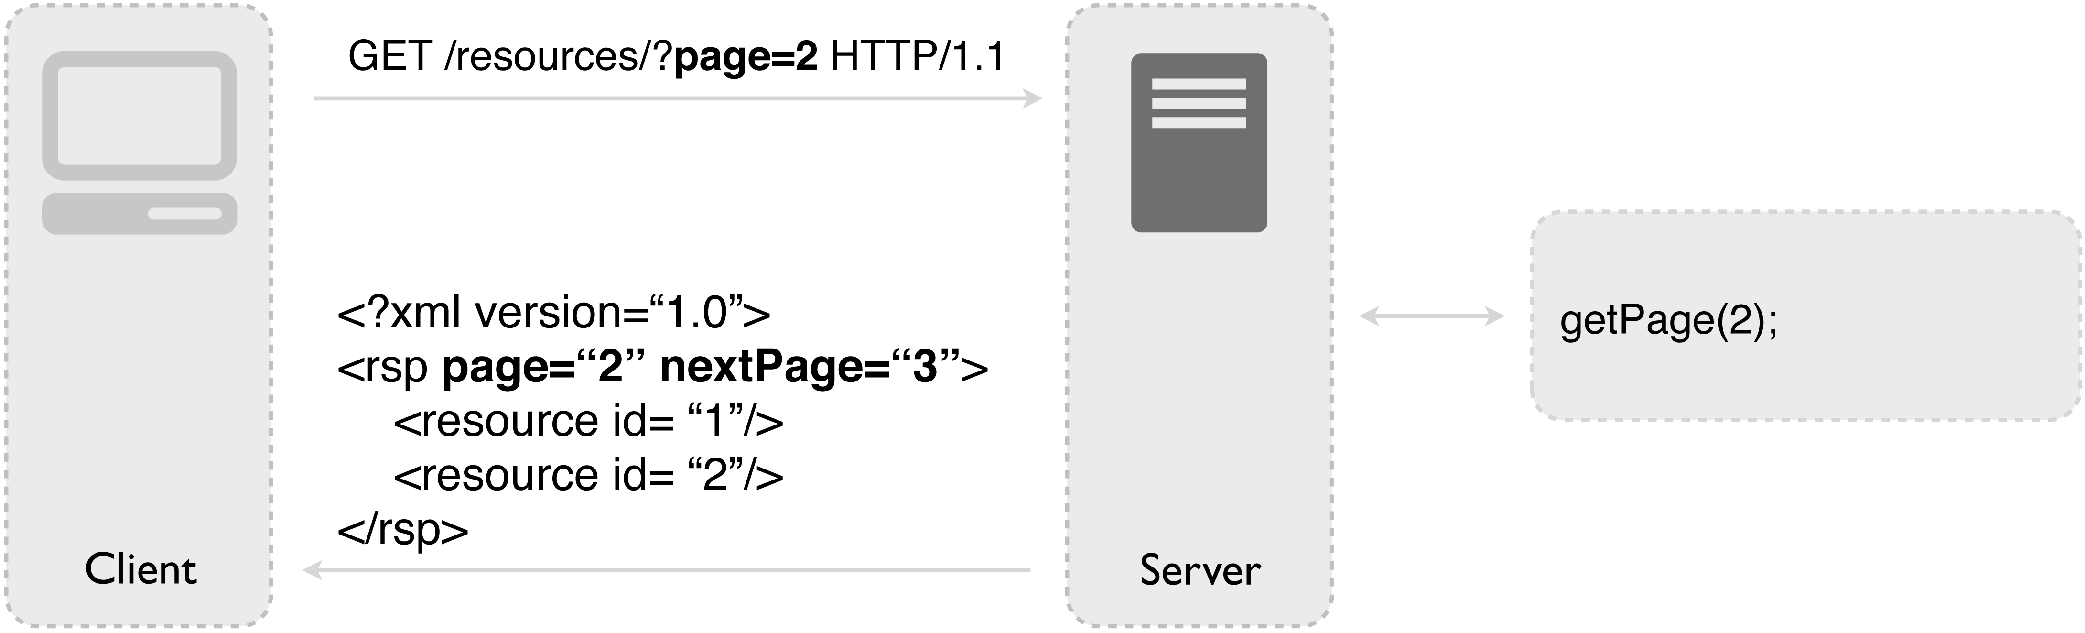
\includegraphics[width=1\textwidth]{images/stateless-design.pdf}
    \caption{Stateless Design}
    \label{fig:stateless-design}
  \end{center}
\end{figure}

As it is illustrated, the request specifies which page the client fetches, i.e. page 2; while the response message contains what the current page is, what the next page is and also the requested page.

On the contrary, stateful design, as shown by Figure \ref{fig:stateful-design} \cite{rodriguez2008restful}, the server saves each client status and responses the corresponding status to the clients who request them. In \ref{fig:stateful-design}, the client need not to specify which page it fetches, but just call the corresponding procedure. The server computes the result and returns the page to the client.

\begin{figure}[ht]
  \begin{center}
    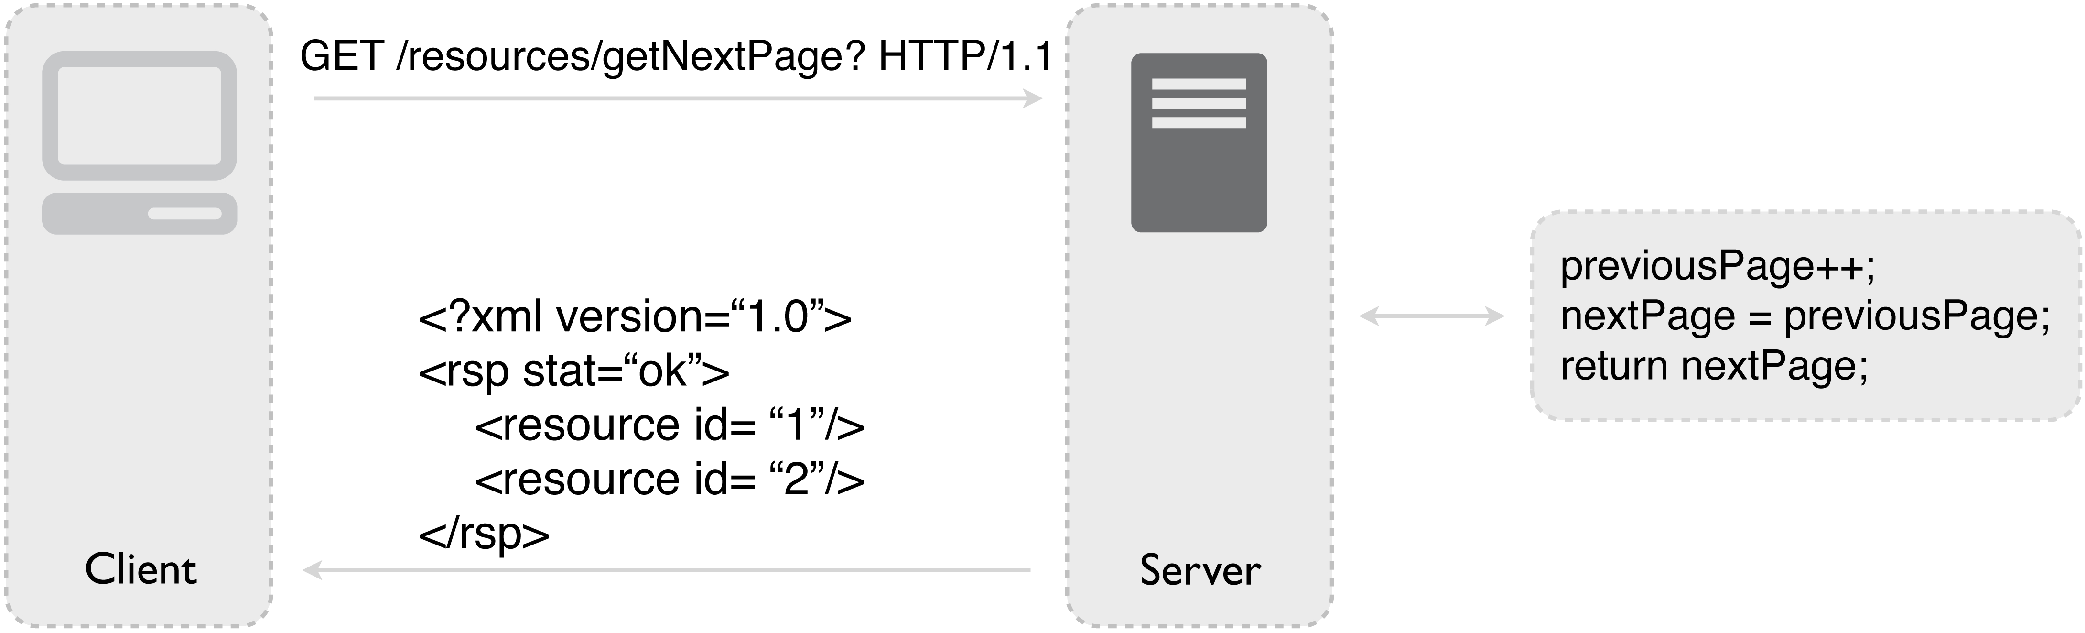
\includegraphics[width=1\textwidth]{images/stateful-design.pdf}
    \caption{Stateful Design}
    \label{fig:stateful-design}
  \end{center}
\end{figure}

The replies are in XML format in Figure \ref{fig:stateless-design} and \ref{fig:stateful-design}, but the REST reply is not restricted in XML document. It could be JSON or other data structure. Usually, REST is implemented relying on HTTP and other web technologies. 

\subsection{SOAP}
SOAP, a protocol designed for web services, specifies, firstly, a XML-based envelope to transfer information; Secondly, a set of rules for translating application and platform-specific data types into XML representations \cite{snell2009programming}. 

SOAP is largely based on XML standards and provides a standard way to structure XML messages. Thus, SOAP has two related applications: Remote Procedure Call (RPC) and Electronic Document Interchange (EDI). RPC is one way to do distributed computing, where one programme calls a function or method (called procedure) on another, optionally with parameters and receiving return value. EDI is used in automated transactions.

A SOAP message contains an optional SOAP header and a required SOAP body. The SOAP header consists of several information blocks and each of the block is a header. Each header explains how the message is to be parsed. The message body is the actual message in XML syntax. 

SOAP provides a mechanism to handle errors which is called SOAP Faults. A SOAP fault consists of fault code, fault string, the fault actor and the fault details. The fault code has been standardised in namespace belong to \url{http://www.w3.org/2001/06/soap-envelope}; The fault string is an explanation of the error for human to read, while the fault detail is a further explanation about the error. The actor is a concept in SOAP Message Exchange Patterns (MEP), a pattern of message exchanged between SOAP nodes, which has been standardised at \cite{booth2007web}.

When a SOAP message is sent from a provider to a receiver, it passes one or more web services. Each of the web service is called intermediary. All these intermediaries that the SOAP message travels through is called a message path. We call each intermediary on a message path an actor. Thus, the fault actor is the unique identifier of message processing node where the error occurs. 

SOAP does not specify the means of SOAP message transports. Generally, SOAP can be transferred through HTTP, FTP, BSD sockets and SMTP etc. 

\subsection{CoAP}
Constrained RESTful Environments (CORE) is a working group under Internet Engineering Task Force (IETF) foaming in 2010\footnote{https://datatracker.ietf.org/wg/core/history/}. CORE has been contributing the major standardisation work for Constrained Application Protocol (CoAP). 

CoAP is a protocol (in draft) used in constrained nodes and constrained networks and designed for machine-to-machine (M2M) applications \cite{shelby2013constrained}. A constrained node, usually, has a lower capacity controller with a small amount of ROM and RAM. Constrained networks refer to the networks, generally, with high packets error rates and a low throughput.

CoAP applications or endpoints interact via a request/response model. It also supports built-in services and resources discoveries. With CoAP, applications or endpoints can easily interact with an HTTP based web architecture \cite{shelby2013constrained}.

Unlike HTTP, CoAP stack is designed for constrained environment, while CoAP, additionally, differ from HTTP in terms of power consumption and overhead. Generally, CoAP power consumption bytes per-transaction are lower than those of HTTP, which implies longer battery lifetime. Figure \ref{fig:http-and-coap-stack} illustrates a comparison between HTTP and CoAP stack. CoAP consists of the concept of HTTP, but it has been re-designed with the respect to the low processing power and energy consumption constraints \cite{colitti2011integrating}.

\begin{figure}[ht]
  \begin{center}
    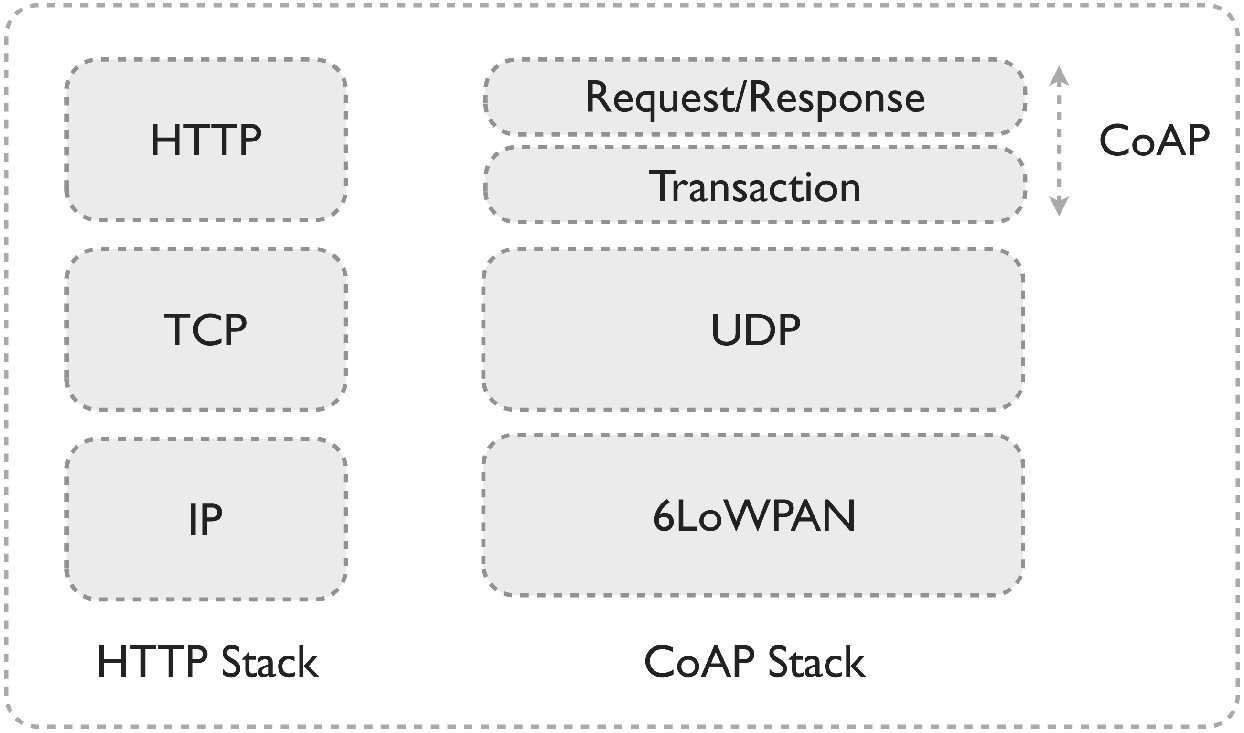
\includegraphics[width=1\textwidth]{images/http-and-coap-stack.pdf}
    \caption{HTTP and CoAP Stack Comparison}
    \label{fig:http-and-coap-stack}
  \end{center}
\end{figure}

CoAP relies on UDP. Moreover, CoAP cannot communicate with a browser directly without a gateway which translates CoAP to HTTP. The gateway can be an application. e.g. Copper\footnote{https://addons.mozilla.org/de/firefox/addon/copper-270430/}, a firefox plug-in, currently, is available for users to browse and interact with Internet of Things devices.

\subsection{MQTT}
Message Queuing Telemetry Transport (MQTT)\footnote{http://mqtt.org} is a machine-to-machine (M2M) / IoT connectivity protocol. There are two main specification for MQTT: MQTT v3.1 and MQTT-S (MQTT for Sensor) v1.2. We will compare MQTT V3.1 with WAMP. Since MQTT-S does not work on TCP/IP network, it is out of scope of our project.

MQTT is designed as an extremely lightweight publish/subscribe messaging transport; while MQTT-S is a publish/subscribe messaging protocol for wireless sensor networks (WSNs) and is originally designed for non-TCP/IP networks.

MQTT V3.1 and WAMP are both working on TCP/IP network. Different from WAMP, MQTT V3.1 assumes the communications channel is more likely to be unreliable.

MQTT V3.1 has a two bytes message header and a UTF8 encoded payload.
Message type, such as Pub/Sub, is defined in the header. Unlike WAMP, MQTT V3.1 does not yet support RPC. Additionally, MQTT V3.1 provides three levels of Quality of Services (QoS) control.

Level 0 is called ``At most once delivery'', when the message is delivered highly dependent to the underlying TCP/IP network. There is no any expectation that the recipient will sent back a response and the message arrives at the recipient at once or it just loses.

Level 1 is called ``At least once delivery'', when a response is expected to be sent back from the recipient, otherwise, the sender will re-send the message.

Level 2 is called ``Exactly once delivery'', when the message will be received and only received once by the recipient. More helper messages will be exchanged at this level to ensure the quality of delivery, and hence there is an increase in the network traffic \cite{MQTTV31ProtocolSpec}.

WAMP, however, does not support such QoS control. Finally, WAMP has been officially registered in the WebSocket Subprotocol Name Registry, while MQTT is not a member.

\subsection{Comparison}
Table \ref{table:WAMPCoAPandMQTTcomparison} is a summary of the comparison between WAMP, CoAP and MQTT.

% If you need to have linefeeds (\\) inside a cell, you must create a new
% paragraph-formatting environment inside the cell. Most common ones are 
% the minipage-environment and the \parbox command (see LaTeX documentation
% for details; or just google for ``LaTeX minipage'' and ``LaTeX parbox'').
\begin{table}
\begin{tabular}{|p{3.3cm}|>{\centering\arraybackslash}p{3cm}|>{\centering\arraybackslash}p{3cm}|>{\centering\arraybackslash}p{3.3cm}|} 
% Alignment of sells: l=left, c=center, r=right. 
% If you want wrapping lines, use p{width} exact cell widths.
% If you want vertical lines between columns, write | above between the letters
% Horizontal lines are generated with the \hline command:
\hline % The line on top of the table
\textbf{ } & \textbf{WAMP} & \textbf{CoAP} & \textbf{MQTT} \\ 
\hline 
% Place a & between the columns
% In the end of the line, use two backslashes \\ to break the line,
% then place a \hline to make a horizontal line below the row 
\textbf{Transport Layer} & TCP & UDP & TCP \\ 
\hline
\textbf{Get Resource} & over WebSockets & HTTP Requests & BSD Sockets \\
% The multicolumn command takes the following 3 arguments: 
% the number of cells to merge, the cell formatting for the new cell, and the
% contents of the cell
\hline
\textbf{Browser} & yes, HTML5 support & no, only via Firefox plugin currently & no, not directly \\
\hline
\textbf{Server} & WebSocket Server with WAMP support & CoAP Server & MQTT Server \\
\hline
\textbf{RPC} & yes & request/response model (through REST APIs) & no \\
\hline
\textbf{Pub/Sub} & yes & yes & yes \\
\hline
\textbf{Proxy Support} & through WebSockets & built-in & external proxy to translate protocol (implies delay) \\
\hline
\end{tabular} % for really simple tables, you can just use tabular
% You can place the caption either below (like here) or above the table
\caption{WAMP, CoAP and MQTT comparison}
\label{table:WAMPCoAPandMQTTcomparison}
\end{table} % table makes a floating object with a title
